\documentclass[11pt, oneside]{article}       % use "amsart" instead of 
\usepackage{geometry}                        % See geometry.pdf to le

\geometry{letterpaper}                           % ... or a4paper or 
%\geometry{landscape}                        % Activate for for  
%\usepackage[parfill]{parskip}            % Activate to begin 
\usepackage{graphicx}                % Use pdf, png, jpg, or eps§ with 
\usepackage{amssymb}
\usepackage{amsmath}
\title{Brief Article}
\author{The Author}
%\date{}                            % Activate to display a given date 

\begin{document}
\maketitle
\section{Introduction}
In this project we tried to design a controller for the Rotary flexible joint. This setup consists of an arm, connected with springs and a joint to a hub, which can rotate in a horizontal plane, driven by a motor. To get an extensive view of the set up we refer to the assignment $\cite[assignment](chapter 2.1)$ for this project. The controller must let the arm track a particular input-function (e.g. a step, or a sine wave) as good as possible. The measured signals are the angle of the hub and the angle of the arm.

The controller we build is based on model-based control system design. So we had to find a state-space model of the system. To do this a lot of mechanical and electrical study has to be done. For a extensive study of the mechanical and electrical part of the Rotary flexible joint we refer again to the assignment $\cite[assignment](chapter 2.1)$. In the assignment the following state-space model is derived: 

\begin{equation}
\begin{pmatrix}
\dot{\theta} \\
\dot{\alpha} \\
\ddot{\theta} \\
\ddot{\alpha} \\
\end{pmatrix}
= \begin{pmatrix}
  0 & 0 & 1 & 0 \\
  0 & 0 & 0 & 1 \\
  0  & \frac{K_{stiff}}{J_h}  & \frac{-K_g^2 K_m K_b}{J_h R_m} & 0 \\
  0 & \frac{-(J_l + J_h)K_{stiff}}{J_h J_l} & \frac{K_g^2 K_m K_b}{J_h R_m} & 0
\end{pmatrix}
\begin{pmatrix}
\theta \\
\alpha \\
\dot{\theta} \\
\dot{\alpha} \\
\end{pmatrix} + 
\begin{pmatrix}
0 \\
0 \\
\frac{K_m K_g}{R_m J_h} \\
\frac{-K_m K_g}{R_m J_h}  \\
\end{pmatrix} V
\end{equation}

The linear state equation can be written in the standard form $\mathbf{\dot{x}} = A \mathbf{x} + B \mathbf{u}$ with our input $\mathbf{u} = V$ and our states $\mathbf{x} = [\theta, \alpha ,\dot{\theta}, \dot{\alpha}]^T$. The output equation has the following standard form $\mathbf{y} = C \mathbf{x}$ with $\mathbf{y} = [\theta, \alpha]^T$. The numerical values for the parameters that we used are stated in the assignment $\cite[assignment](chapter 6)$. The numerical values of the matrices $A,B,C$ and $D$ are stated below.
\begin{equation}
A = 
\begin{pmatrix}
  0 & 0 & 1 & 0 \\
  0 & 0 & 0 & 1 \\
  0  & 765.9810  & -52.7952 & 0 \\
  0 & -1038.618 & 52.7952 & 0
\end{pmatrix} \hspace{0.5cm}
B = 
\begin{pmatrix}
  0 \\
  0 \\
  98.3333 \\
  -98.3333
\end{pmatrix} \hspace{0.5cm}
C = 
\begin{pmatrix}
  1 & 0 & 0 & 0 \\
  0 & 1 & 0 & 0 
\end{pmatrix} \hspace{1cm}
\end{equation}

We performed a short open loop analysis of the system. The poles of the open loop system are $0,-8.9761+18.2356i,-8.9761-18.2356i$ and $-34.8429$. Because the poles are all in complex left half plane, we can say that our open loop system is stable. Therefore our system is also stabilizable. The open loop system has no transmission zeros. The ranks of the controllability and observability matrices both equals $4$ where $4$ is the number of states. Hence our system is controllable and observable. From this only we can already conclude that the system is minimal. When we checked it in Matlab, it was indeed so. 
\newline
\newline
The control goals for our controller are to accurately track the setpoints, to give a fast response, to give a good disturbance rejection. Of course the closed loop system should also be stable.





\section{Tests of the controller on the real setup}

\begin{figure} \label{realtimeSimDiagram}
  \centering
  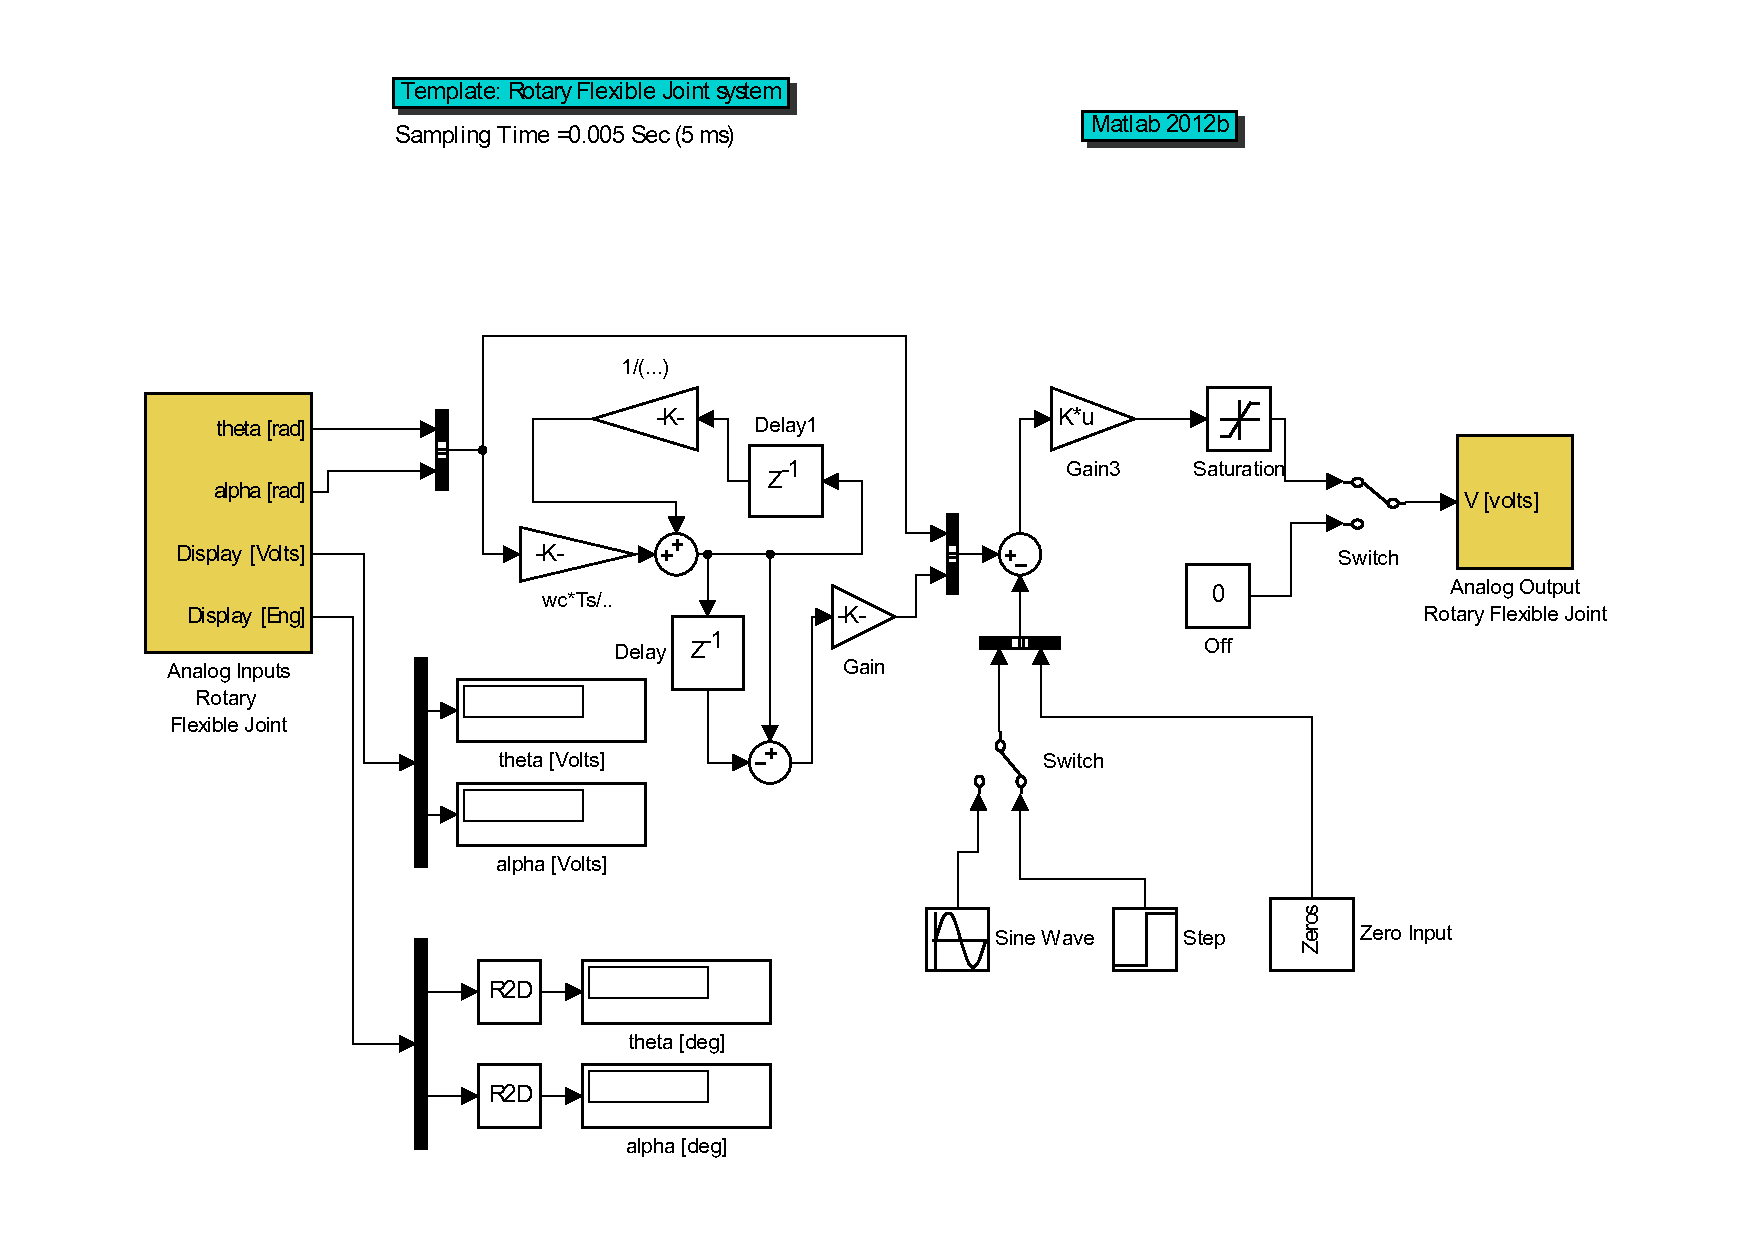
\includegraphics[scale=0.6]{realtimeSimDiagram}
  \caption{Real-time Simulink diagram} 
\end{figure}

In figure $\eqref{realtimeSimDiagram}$ we see the real-time Simulink diagram that we used in the lab for the real setup. The "Analog Inputs" block gives the measurements of the sensors (they are updated each 5 ms) in radians for the angles of the hub and the arm. Additionally this block has two special outputs, "Display[volts]" and "Display[Eng]", which are used for visualization purposes. These two outputs are connected to a set of displays in order to provide a local visual measure of the process variables. 

The "Analog Output" block allows the controller to send a voltage signal to the motor of the hub. At the input of this block there is an on-off switch. This switch allows you to switch on or switch off the motor. We included a saturator in our diagram just before the signal goes in to the "Analog Output" block because the output voltage is limited from $-5V$ to $5V$. The saturator settings in our diagram are set accordingly. You can also see a sin wave, a step input and a zero input. These are used to represent a reference signal for the output. The sine wave or the step input is the reference for $\theta_{desired}$ and the zero block are 3 signals equals to zero that represent the reference for $\alpha, \dot{\theta}$ and $\dot{\alpha}$.



\begin{thebibliography}{99}
\bibitem{assignment}
Oscar Mauricio Adegulo , Bart De Moor (2014). CACSD Practicum Session Rotary Flexible Joint.
% \bibitem{art1}
% Pierce, Rod. (3 Feb 2014). ``Math is Fun - Maths Resources". Math Is Fun. Retrieved 13 Mar 2014 from http://www.mathsisfun.com/index.htm
\end{thebibliography}
\end{document}






